\documentclass[a4paper, 11pt]{article}
\usepackage{graphicx} % Required for inserting images
\usepackage{amsmath,amssymb,amsthm,enumerate,nicefrac,fancyhdr,hyperref,adjustbox}

\newcommand{\cv}[1]{\begin{pmatrix} #1 \end{pmatrix}}
\title{The Exploration of Harmonic Motion and The Journey to Nonlinear Mechanics}
\author{Evan Bayer, Jesús Minakata Mata, Vaughn Gerrits}
\date{November 2023}

\begin{document}
\maketitle
\tableofcontents
https://www.overleaf.com/project/65495705fa74644eaca189bd

\section{Introduction}
The Exploration and study of Harmonic Motion can give us an insight into how different physical systems work and knowledge about our world. We begin our story at the simplest problem, the problem that gives rise to the phenomena known as Simple Harmonic Motion. 

\subsection{Hooke's Law}
Hooke's Law is very simple, it states the Restoring Force of a spring is proportional to the distance from the equilibrium position. 

$$F_{Spring} = -kx$$

Where k is the spring constant, and x is the distance from the equilibrium position.

\subsection{Frictionless Spring}
Consider the following mass on the end of a spring confined to move in the x-direction on a friction-less surface:

\begin{center}
    \centering
    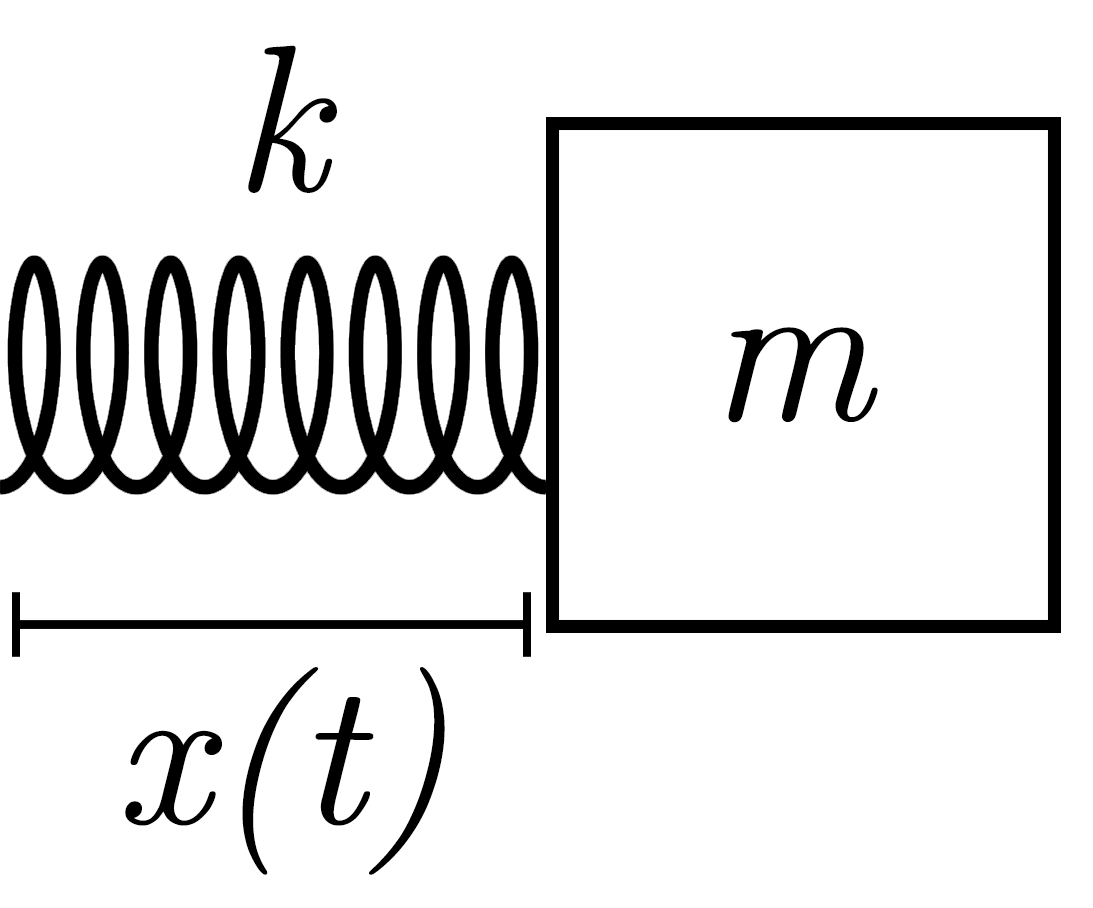
\includegraphics[width=0.25\linewidth]{SHO.png}
    \label{fig:enter-label}
\end{center}

Newtons 2nd Law yields:

$$F_{net} = m\ddot{x}(t) = -kx(t)$$
Where: 
$$\dot{x}(0) = 0 \;\;\;\;\;\; x(0) = x_0$$
Let
$$ v = \frac{dx}{dt}$$
Then
$$ \frac{d}{dx}v = \frac{d}{dx}\frac{dx}{dt} = \ddot{x} = \frac{dv}{dx}\frac{dx}{dt} = \frac{dv}{dx}v $$
$$ m\int{v}\,{dv} = -k\int x\,dx $$
$$ v = \sqrt{\frac{k}{m}}xi $$
$$ x(t) = e^{\sqrt{\frac{k}{m}}ti} $$
Let $$ \omega = \sqrt{\frac{k}{m}} $$
$$ x(t) = A\cos{\omega t} + B\sin{\omega t} $$
$$ x'(t) = -A\omega \sin{\omega t} + B\omega \cos{\omega t} $$
$$ x(0) = x_0 = A $$
$$ x'(0) = 0 = B\omega \; ; \; B = 0 $$


\section{Simple Pendulum}
Consider the following mass m attached to a massless string of fixed length l subject to the earth gravitational field .on the end of a string subject to gravity. 
\begin{center}
    \centering
    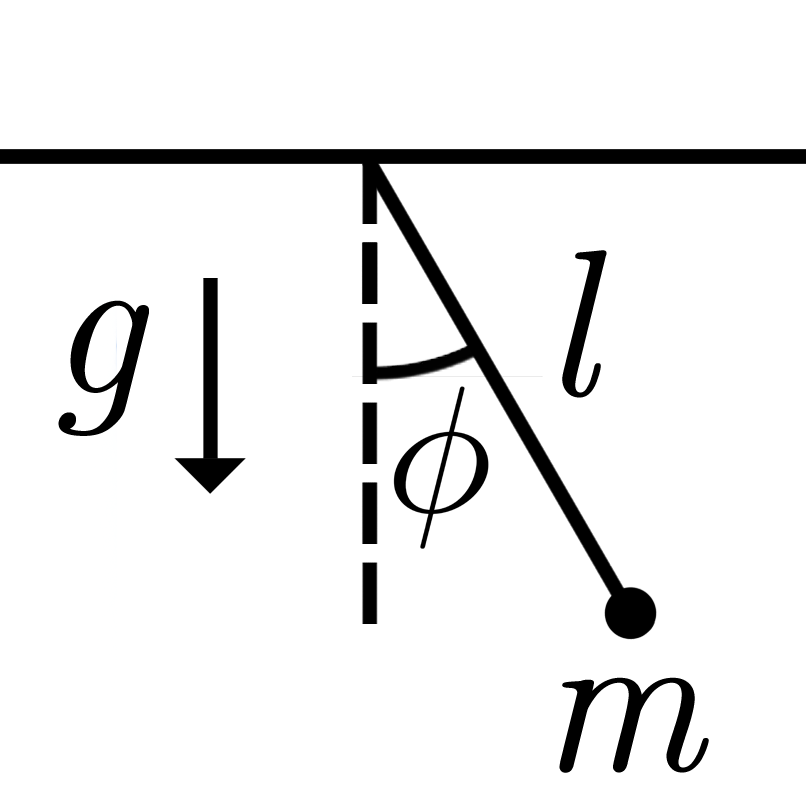
\includegraphics[width=0.25\linewidth]{simplependulum.png}
    \label{fig:enter-label}
\end{center}
as we saw in class we can use define a Lagrangian for the system and use the Euler Lagrange equations to derive the following equation of motion,
$$\ddot{\phi} + \frac{g}{l}sin\phi = 0$$
let $u = \dot{\phi}$ :
$$\begin{cases}
    \dot{\phi} = u \\
    \dot{u} = -\frac{g}{l} sin\phi
\end{cases}$$ \\
which is a system of ODE's and can be written in vector form as
$$\cv{\dot{\phi} \\\dot{u}} = \cv{ u \\ -\frac{g}{l} sin\phi}$$
now lets define $\bf{X} = \cv{\phi \\ u} $  \ such that, 
$$\frac{d\bf{X}}{dt} = \cv{ u \\ -\frac{g}{l} sin\phi}$$
\section{Double Pendulum}
Consider the following mass on the end of a string attached to another mass on a string, both subject to gravity.
\begin{center}
    \centering
    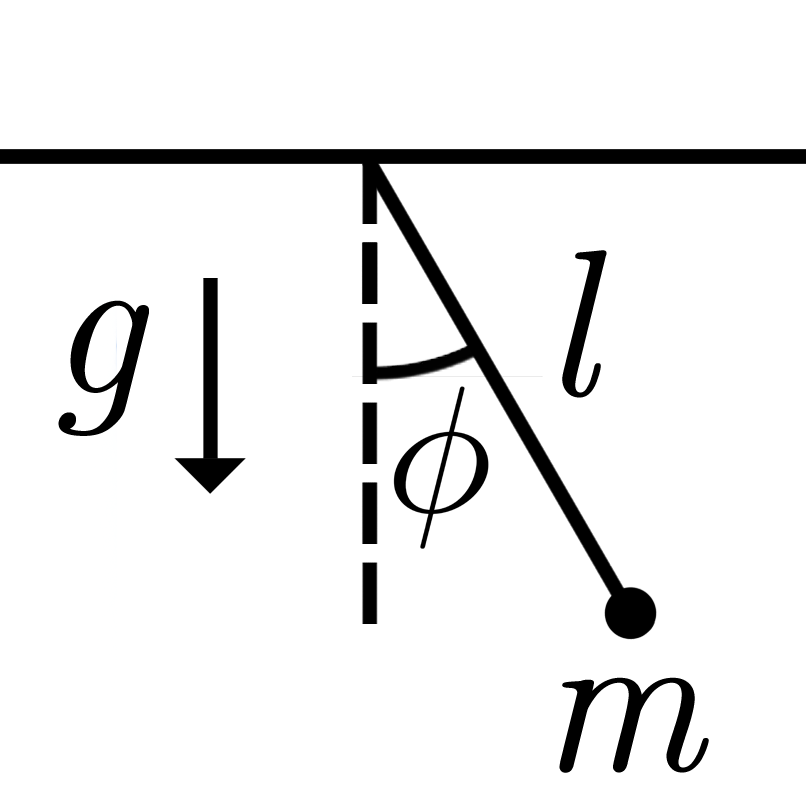
\includegraphics[width=0.25\linewidth]{simplependulum.png}
    \label{fig:enter-label}
\end{center}
the introduction of the second pendulum into the system is a simple change that results in a much more chaotic system. this system is still conservative however, so we can use the Lagrangian as we normally would

$$T=\frac{1}{2}[m_1 l_1^2 \dot{\phi}_1^2 + m_2(l_1^2 \dot{\phi}_1^2 + l_2^2 \dot{\phi}_2^2 + 2l_1 l_2 \dot{\phi}_1 \dot{\phi}_2\cos(\phi_1 - \phi_2))]$$
$$U=-g[(m_1+m_2)l_1\cos(\phi_1)+m_2l_2\cos(\phi_2)]$$
$$\mathcal{L}=T-U$$

and from the Lagrangian, we get the 2 Euler-Lagrange equations of motion for this system

$$-m_2l_1 l_2 \dot{\phi}_1 \dot{\phi}_2 \sin(\phi_1 - \phi_2) - g(m_1 + m_2)l_1\sing(\phi_1)=0$$

\section{Damped Driven Double Pendulum}
\begin{center}
    \centering
    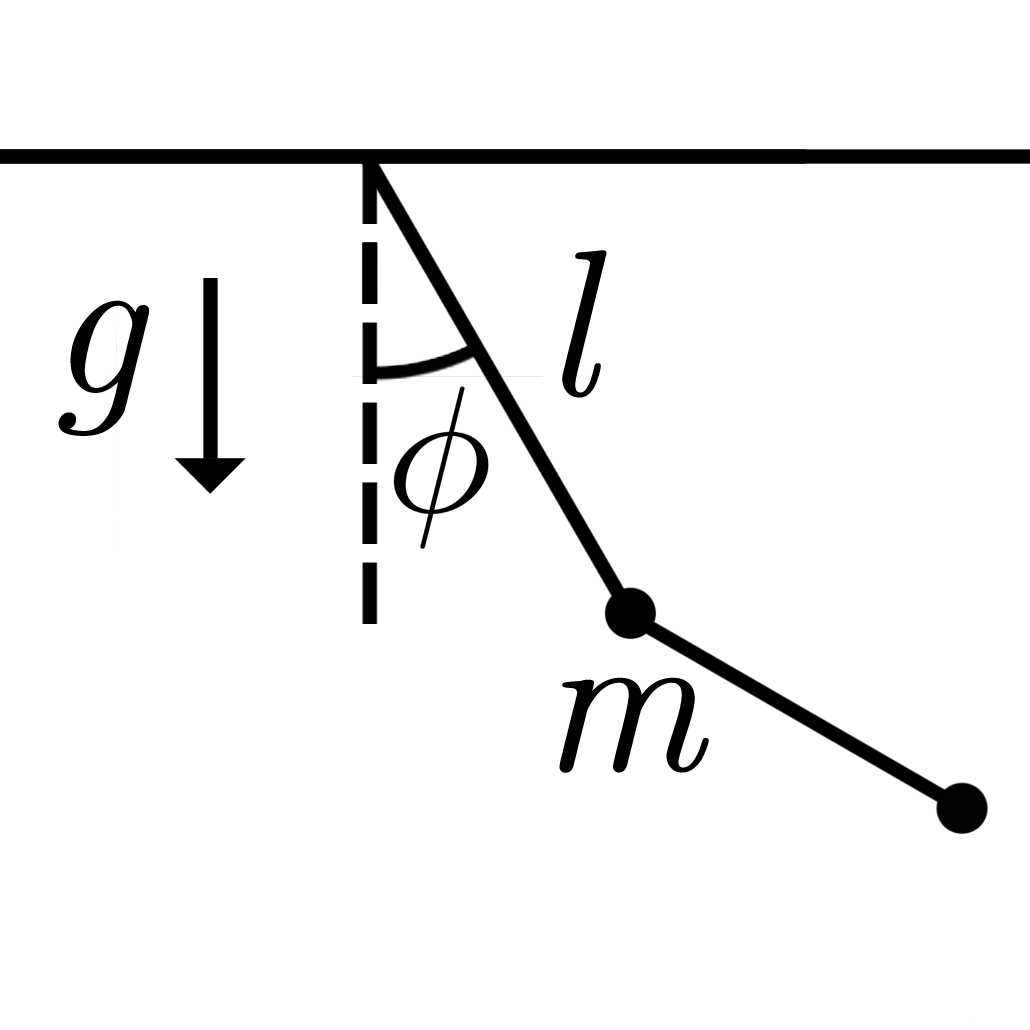
\includegraphics[width=0.25\linewidth]{doublependulum.png}
    \label{fig:enter-label}
\end{center}




\end{document}
